\documentclass[journal]{IEEEtran}
\input{settings}
\begin{document}

\section{既存のウェブセキュリティモデルにおける時相論理}
本章では、本研究の提案モデルの拡張元である二つの既存ウェブセキュリティモデルの時相論理の表現能力と問題点を述べる。

\subsection{基礎モデル}
\label{sec:based-model}
Akhaweらによって提案されたウェブセキュリティモデル\cite{based-model}は、リクエストやレスポンスといったイベントの発生順序を表すための時間軸を表す時相論理を実装している。
まず、時間軸となるTimeクラスをCode\ref{code:time}のように記述する。
\begin{lstlisting}[caption=基礎モデルにおける時間軸, label=code:time]
open util/ordering[Time]

sig Time {}

fact Traces{
	all t:Time- last | one e:Event | e.pre=t and e.post=t.next
	all e:Event | e.post=e.pre.next
}
\end{lstlisting}
Timeクラスのインスタンスはorderingのオプションにより順序付けが可能となり、次の順番のインスタンスを表すnext演算子、インスタンスの並びで最初と最後のインスタンスを表すfirst,lastといった演算子が使用できる。
このTimeクラスにリクエストやレスポンスを表すEventクラスを関連付けることで、発生するイベントの順序をTimeクラスの時間軸で表すことができる。

\subsection{Cookieを包括するモデル}
\label{sec:cookie-model}
Ryckらによって提案されたウェブセキュリティモデル\cite{cookie-model}は、基礎モデルで導入したイベントの時間軸を応用し、イベント発生時のCookieの状態変化を表現できるよう時相論理を拡張している。
Cookieに対しての時相論理はCode\ref{code:cookie-model-temporal-logic}に示すコードで実装される。
\begin{lstlisting}[caption=Cookieに対する時相論理, label=code:cookie-model-temporal-logic]
sig CSState {
	dst: Origin,
	cookies: set Cookie
}

sig CSStateHTTPTransaction extends HTTPTransaction {
	beforeState: CSState,
	afterState: CSState
}{
	beforeState.dst = afterState.dst
	afterState.cookies = beforeState.cookies + (resp.headers & SetCookieHeader).thecookie
	
	beforeState.dst = req.host
}
\end{lstlisting}
まず、Cookieの状態変化を表現するために各時点でのCookieの状態を表現するクラスが必要となるので、これをCSStateとして定義する。
これを対応するリクエストとレスポンスを表現するHTTPTransactionクラスに関連付けることで、リクエスト時とレスポンス時のブラウザ内のCookieの状態を表現できる。
また、リクエスト時とレスポンス時の状態間でCookieの集合がどのように変化するか表現している。
したがって、Code\ref{code:cookie-model-temporal-logic}の記述により、対応するリクエストとレスポンスの間で発生するCookieの状態変化を表現している。

\subsection{既存モデルにおける問題点}
\label{sec:existing-models-problems}
\ref{sec:based-model}、\ref{sec:cookie-model}節の二つの既存モデルの時相論理の表現能力には問題点がある。
それぞれの既存モデルの時相論理の表現能力を以下に整理する。
\begin{itemize}
\item 基礎モデル \\
リクエストやレスポンスの発生順序を表現するための時間軸を表現できる。
\item Cookieモデル \\
対応するリクエストとレスポンス間でのCookieの状態変化を表現できる。
\end{itemize}
これらの時相論理の能力では、状態変化は対応するリクエストとレスポンス間でのみ表現することができ、異なる通信の状態クラスにその内容を引き継ぐことはできない。
つまり、3状態以上の遷移を含む状態変化を表現できない。
具体的には図\ref{fig:2transaction-a}のような状況が考えられる。
図\ref{fig:2transaction-a}は、ある同一のブラウザからリクエストが二つ連続して送信され、送信したリクエストに対するレスポンスが順番に発生した状況を表している。
Cookieモデルでの表現能力では、図\ref{fig:2transaction-a}内で示している通りCSState1からCSState3へ、CSState2からCSState4への保有するCookieの集合の変化を表現できる。
しかし、この表現能力ではCSState3で格納されたCookie1がCSState4で格納されていること(図\ref{fig:2transaction-b}のような状態)は起こりえない。
なぜなら、CSState4はCSState3で生じた状態変化を捉えることができないためである。
しかし、実際のCookieの動作を考えると、図\ref{fig:2transaction-b}に示す状態が表現されるべきである。
本研究ではこのように時間軸に沿った状態変化をAlloyで実現するための記述法を提案する。

\begin{figure}[htb]
\centering
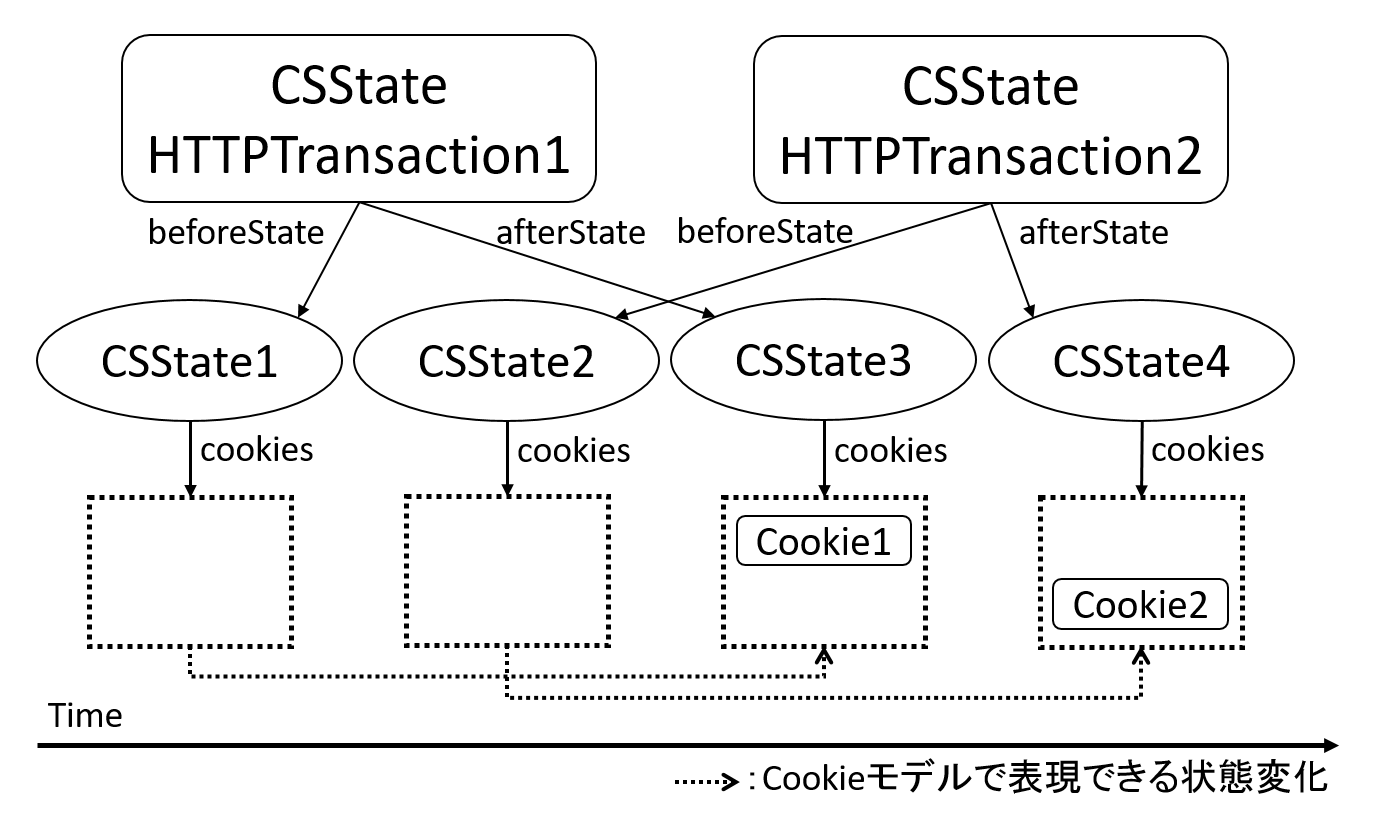
\includegraphics[width=\hsize]{./fig/2transaction-a.eps}
\caption{Cookieモデルで表現可能な状態変化の一例}
\label{fig:2transaction-a}
\end{figure}

\begin{figure}[hbt]
\centering
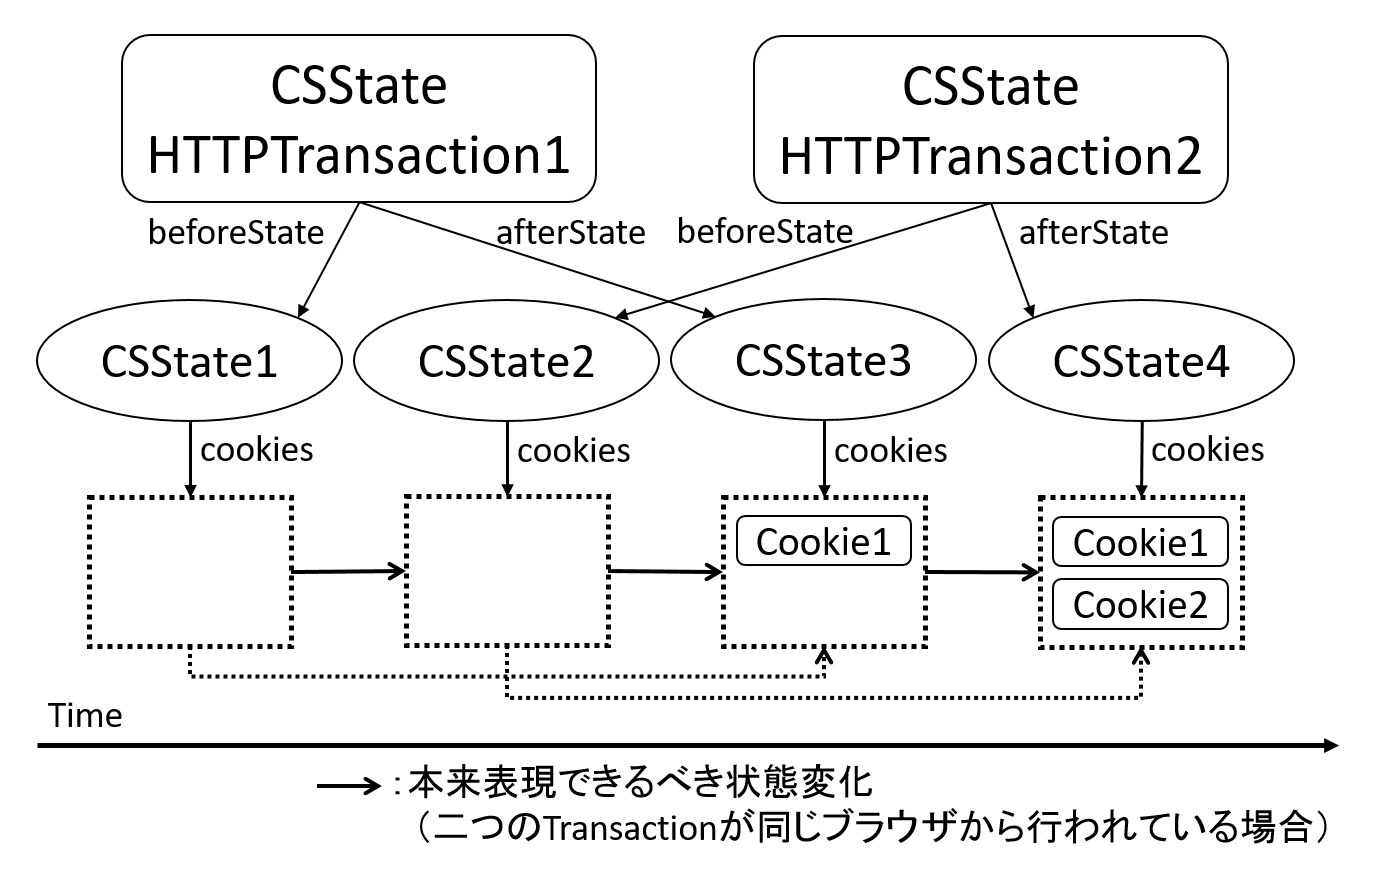
\includegraphics[width=\hsize]{./fig/2transaction-b.eps}
\caption{Cookieモデルで表現不可能な状態変化の一例}
\label{fig:2transaction-b}
\end{figure}

\end{document}
